\documentclass{beamer}

\newcommand\tab[1][1cm]{\hspace*{#1}}
\usepackage[spanish]{babel}
\usepackage[utf8]{inputenc}
\usepackage{bussproofs}
\usepackage{url}
\usepackage[document]{ragged2e}
\usepackage{tikz}
\usetikzlibrary{shapes,arrows,spy,positioning,snakes}
\usepackage{verbatim} % comentarios
\usepackage{tabulary} % tablas

\DeclareOptionBeamer{compress}{\beamer@compresstrue}
\ProcessOptionsBeamer

\mode<presentation>

\useoutertheme[footline=authortitle]{miniframes}
\useoutertheme{infolines}
\useinnertheme{circles}
\usecolortheme{whale}
\usecolortheme{orchid}

\definecolor{beamer@blendedblue}{rgb}{0.137,0.466,0.741}

\setbeamercolor{structure}{fg=beamer@blendedblue}
\setbeamercolor{titlelike}{parent=structure}
\setbeamercolor{frametitle}{fg=black}
\setbeamercolor{title}{fg=black}
\setbeamercolor{item}{fg=black}

\setbeamertemplate{bibliography item}[text]

\mode
<all>

\title[]{Commercial paper}
\subtitle{Fundamentos de blockchains}
\author{René Dávila - Jorge Solano}
%\institute{IIMAS}
\date{ }

\AtBeginSection[] { 
	\begin{frame} 
		\frametitle{Índice}
		\tableofcontents[currentsection]
	\end{frame}
}
\AtBeginSubsection[] { 
	\begin{frame}
		\frametitle{Índice}
		\tableofcontents[currentsection, currentsubsection]
	\end{frame}
}

\setbeamertemplate{navigation symbols}{}

\begin{document}
	\EnableBpAbbreviations
	
	\begin{frame}
		\begin{center}
			
\includegraphics [width =0.2 \textwidth ]{iimas}
		\end{center}
		\titlepage 
	\end{frame}

	\section{Commercial paper}
	
	\begin{frame}
		Diagrama de las organizaciones:
		\begin{figure}[h]
			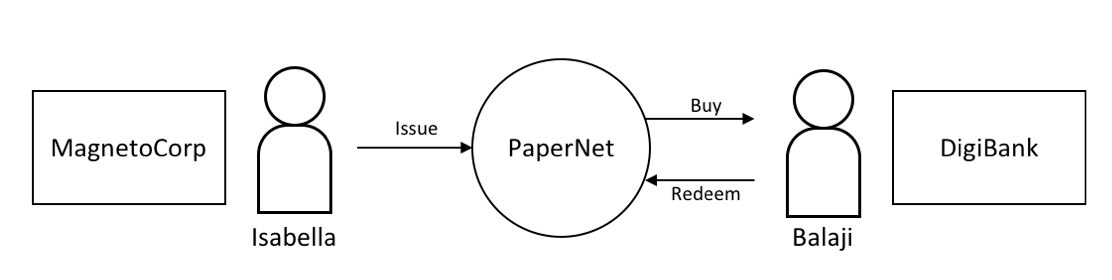
\includegraphics[scale=.5]{papernet_01}
			\centering
		\end{figure}
		Las organizaciones MagnetoCorp y DigiBank intercambian papeles comerciales en la red PaperNet.
	\end{frame}
	
	\subsection{PaperNet}

	\begin{frame}
		\frametitle{Peers y canal de comunicación}
		En cd fabric-samples/test-network:\\
		\begin{center}
			\begin{tabulary}{\linewidth}{L}
				\hline
				(PaperNet admin)\$ ./network.sh up \\
				\hline 
				(PaperNet admin)\$ ./network.sh createChannel \\
				\hline
			\end{tabulary} 
		\end{center}
	\end{frame}
	
	\begin{frame}
		\frametitle{Red docker net\_test}
		En cd fabric-samples/commercial-paper\\
		\begin{center}
			\begin{tabulary}{\linewidth}{L}
				\hline
				(PaperNet admin)\$ ./network-starter.sh \\
				\hline 
				(PaperNet admin)\$ docker ps \\
				\hline
				(PaperNet admin)\$ docker network inspect net\_test \\
				\hline
			\end{tabulary} 
		\end{center}
		peer0.org1.example.com $\rightarrow$ DigiBank\\
		peer0.org2.example.com $\rightarrow$ MagnetoCorp
	\end{frame}

	\begin{frame}
		\frametitle{Monitor de la red}
		En cd commercial-paper/organization/magnetocorp\\
		\begin{center}
			\begin{tabulary}{\linewidth}{L}
				\hline
				(MagnetoCorp admin)\$ ./monitordocker.sh net\_test \\
				\hline
			\end{tabulary} 
		\end{center}
	\end{frame}
	
	\subsection{Crear smart contract propio (MagnetoCorp)}
	
	\begin{frame}
		\frametitle{Código del smart contract}
		En cd commercial-paper/organization/magnetocorp\\
		\begin{center}
			\begin{tabulary}{\linewidth}{L}
				\hline
				(MagnetoCorp dev)\$ code contract \\
				\hline
			\end{tabulary} 
		\end{center}
	\end{frame}

	\begin{frame}
		\frametitle{Ciclo de vida en Fabric}
		\begin{figure}[h]
			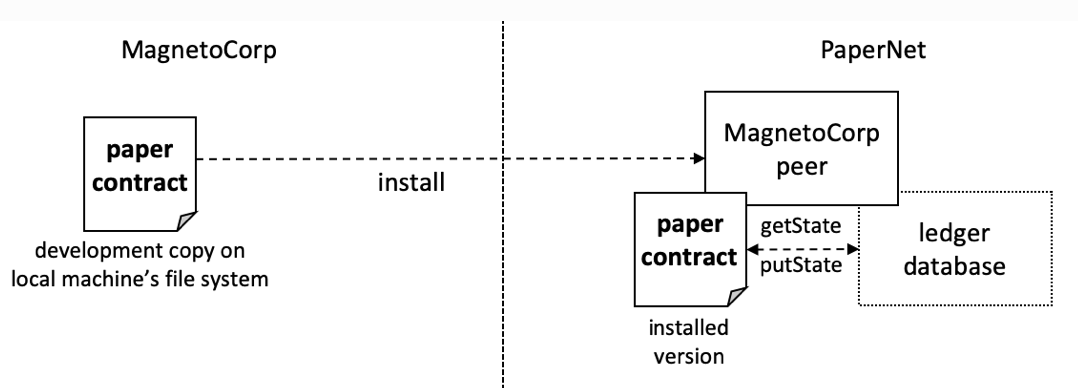
\includegraphics[scale=.4]{papernet_02}
			\centering
		\end{figure}
		\begin{itemize}
			\item El desarrollador empaqueta el chaincode ([1...n] smart contract)
			\item El administrador instalar el chaincode en cada organización.
			\item El administrador de cada organización debe aprobar el chaincode.
			\item El administrador publica en el chaincode en el ledger del canal asociado.
		\end{itemize}
		{\tiny \url{https://hyperledger-fabric.readthedocs.io/en/release-2.0/chaincode\_lifecycle.html\#chaincode-lifecycle} }
	\end{frame}
	
	\begin{frame}
		\frametitle{Instalación y aprobación}
		\textbf{Variables de entorno:} En cd commercial-paper/organization/magnetocorp hay que establecer las variables de entorno para que el administrador pueda instalar y aprobar el chaincode en la organización MagnetoCorp.\\
		\begin{center}
			\begin{tabulary}{\linewidth}{L}
				\hline
				(MagnetoCorp admin)\$ source magnetocorp.sh\\
				\hline
			\end{tabulary} 
		\end{center}
	\end{frame}
	
	\begin{frame}
		\frametitle{Instalación y aprobación}
		\textbf{Empaquetar chaincode:} El smart contract se puede empacar en un chaincode utilizando el comando peer lifecycle chaincode package.\\
		\begin{center}
			\begin{tabulary}{\linewidth}{L}
				\hline
				(MagnetoCorp admin)\$ peer lifecycle chaincode package cp.tar.gz --lang node --path ./contract --label cp\_0\\
				\hline
			\end{tabulary} 
		\end{center}
	\end{frame}
	
	\begin{frame}
		\frametitle{Instalación y aprobación}
		\textbf{Instalar chaincode:} El smart contract se puede instalar utilizando el comando peer lifecycle chaincode install.\\
		\begin{center}
			\begin{tabulary}{\linewidth}{L}
				\hline
				(MagnetoCorp admin)\$ peer lifecycle chaincode install cp.tar.gz\\
				\hline
			\end{tabulary} 
		\end{center}
	\end{frame}
	
	\begin{frame}
		\frametitle{Instalación y aprobación}
		\textbf{Aprobar chaincode:} MagnetoCorp debe aprobar el papercontract que se acaba de instalar con el package ID del contrato.\\
		\begin{center}
			\begin{tabulary}{\linewidth}{L}
				\hline
				(MagnetoCorp admin)\$ peer lifecycle chaincode queryinstalled \\
				\hline
				(MagnetoCorp admin)\$ export PACKAGE\_ID=cp\_0:ffda9... \\
				\hline
				(MagnetoCorp admin)\$ peer lifecycle chaincode approveformyorg --orderer localhost:7050 --ordererTLSHostnameOverride orderer.example.com --channelID mychannel --name papercontract -v 0 --package-id \$PACKAGE\_ID --sequence 1 --tls --cafile \$ORDERER\_CA \\
				\hline
			\end{tabulary} 
		\end{center}
	\end{frame}
	
	\subsection{Aprobar smart contract ajeno (DigiBank)}
	
	\begin{frame}
		\frametitle{Instalación y aprobación}
		Por defecto, el ciclo de vida del chaincode en Fabric requiere que la mayoría de las organizaciones apruebe la definición de un chaincode en el canal. En este caso, se tienen 2 organizaciones, por lo tanto, se requiere que las 2 organizaciones apruebe el chaincode.
	\end{frame}
	
	\begin{frame}
		\frametitle{Instalación y aprobación}
		\textbf{Variables de entorno:} En cd commercial-paper/organization/digibank/ hay que establecer las variables de entorno para que el administrador de DigiBank pueda instalar y aprobar el papernet chaincode.\\
		\begin{center}
			\begin{tabulary}{\linewidth}{L}
				\hline
				(DigiBank admin)\$ source digibank.sh\\
				\hline
			\end{tabulary} 
		\end{center}
	\end{frame}
	
	\begin{frame}
		\frametitle{Instalación y aprobación}
		\textbf{Empaquetar chaincode:} El smart contract se puede empacar en un chaincode utilizando el comando peer lifecycle chaincode package.\\
		\begin{center}
			\begin{tabulary}{\linewidth}{L}
				\hline
				(DigiBank admin)\$ peer lifecycle chaincode package cp.tar.gz --lang node --path ./contract --label cp\_0\\
				\hline
			\end{tabulary} 
		\end{center}
	\end{frame}
	
	\begin{frame}
		\frametitle{Instalación y aprobación}
		\textbf{Instalar chaincode:} El smart contract se puede instalar utilizando el comando peer lifecycle chaincode install.\\
		\begin{center}
			\begin{tabulary}{\linewidth}{L}
				\hline
				(DigiBank admin)\$ peer lifecycle chaincode install cp.tar.gz\\
				\hline
			\end{tabulary} 
		\end{center}
	\end{frame}
	
	\begin{frame}
		\frametitle{Instalación y aprobación}
		\textbf{Aprobar chaincode:} DigiBank debe aprobar el papercontract que se acaba de instalar con el package ID del contrato.\\
		\begin{center}
			\begin{tabulary}{\linewidth}{L}
				\hline
				(DigiBank admin)\$ peer lifecycle chaincode queryinstalled \\
				\hline
				(DigiBank admin)\$ export PACKAGE\_ID=cp\_0:ffda9... \\
				\hline
				(DigiBank admin)\$ peer lifecycle chaincode approveformyorg --orderer localhost:7050 --ordererTLSHostnameOverride orderer.example.com --channelID mychannel --name papercontract -v 0 --package-id \$PACKAGE\_ID --sequence 1 --tls --cafile \$ORDERER\_CA \\
				\hline
			\end{tabulary} 
		\end{center}
	\end{frame}
	
	\subsection{Publicar smart contract (DigiBank)}
	
	\begin{frame}
		\frametitle{Publicación}
		Una vez que el contrato ha sido aprobado por la mayoría del consorcio (2/2) en el canal, se crea un nuevo contenedor docker para ejecutar el papercontract en los nodos de la red y así, éste pueda ser invocado por las aplicaciones cliente en el canal.
	\end{frame}

	\begin{frame}
		\frametitle{Instalación y aprobación}
		\textbf{Publicar papercontract:} Ya aprobado, el administrador de cualquier organización puede publicar el smart contract utilizando el comando peer lifecycle chaincode commit.\\
		\begin{center}
			\begin{tabulary}{\linewidth}{L}
				\hline
				(DigiBank admin)\$ peer lifecycle chaincode commit -o localhost:7050 --ordererTLSHostnameOverride orderer.example.com --peerAddresses localhost:7051 --tlsRootCertFiles \${PEER0\_ORG1\_CA} --peerAddresses localhost:9051 --tlsRootCertFiles \${PEER0\_ORG2\_CA} --channelID mychannel --name papercontract -v 0 --sequence 1 --tls --cafile \$ORDERER\_CA --waitForEvent\\
				\hline
			\end{tabulary} 
		\end{center}
	\end{frame}
	
	\subsection{Emitir un papel comercial (MagnetoCorp)}
	
	\begin{frame}
		\frametitle{Diagrama para la emisión}
		Para emitir el papel comercial MagnetoCorp utiliza su aplicación cliente llamada issue.js.
		\begin{figure}[h]
			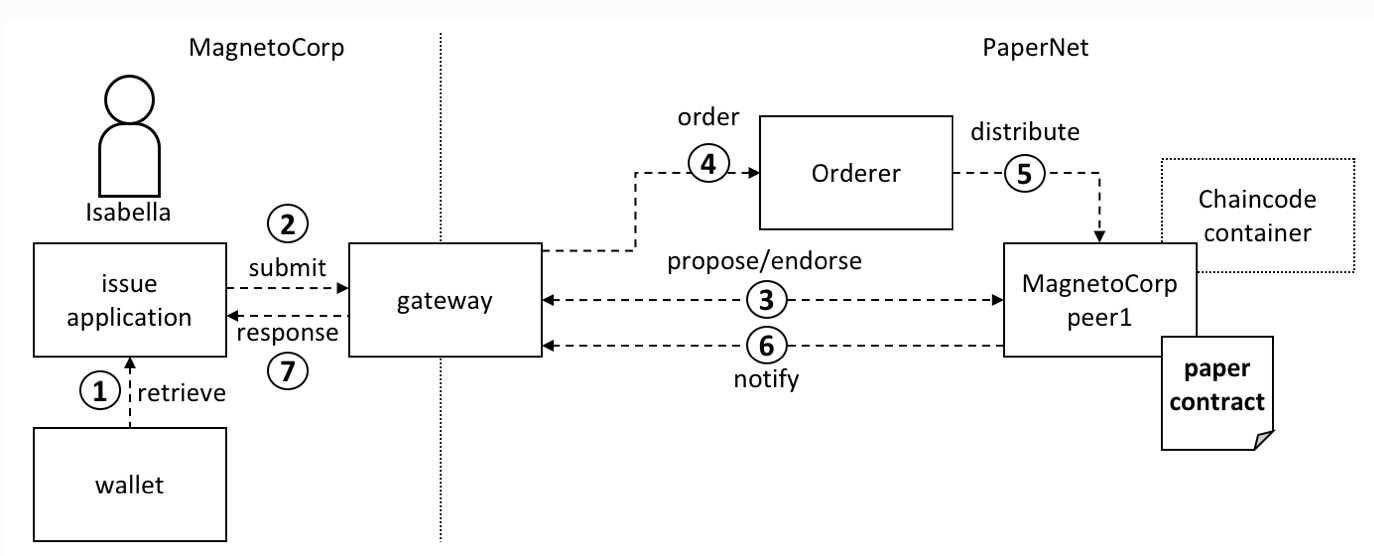
\includegraphics[scale=.4]{papernet_03}
			\centering
		\end{figure}
	\end{frame}
	
	\begin{frame}
		\frametitle{Emisión}
		En cd commercial-paper/organization/magnetocorp/application/ se pueden ver los archivos \textbf{addToWallet.js}, \textbf{issue.js} y \textbf{package.json}.\\
		\vspace{4mm}
		Isabella va a utilizar addToWallet.js para agregar su identidad al wallet (Certificado X.509). issue.js utilizará esa identidad para crear el papel comercial a nombre de MagnetoCorp invocando al papercontract.
	\end{frame}
	
	\begin{frame}
		\frametitle{Emisión}
		Como se puede observar al inicio del archivo \textbf{issue.js} se requieren ciertas dependencias las cuales están declaras en el archivo \textbf{package.json} y se pueden descargar con npm.\\
		\begin{center}
			\begin{tabulary}{\linewidth}{L}
				\hline
				(Isabella)\$ npm install \\
				\hline
			\end{tabulary} 
		\end{center}
	\end{frame}
	
	\begin{frame}
		\frametitle{Emisión}
		Ahora, Isabella debe agregar su credenciales X.509 a su wallet.\\
		\begin{center}
			\begin{tabulary}{\linewidth}{L}
				\hline
				(Isabella)\$ node addToWallet.js \\
				\hline
				(Isabella)\$ ls ../identity/user/isabella/wallet/ \\
				\hline
			\end{tabulary} 
		\end{center}
	\end{frame}
	
	\begin{frame}
		\frametitle{Emisión}
		Ahora sí, Isabella puede utilizar \textbf{issue.js} para enviar la transacción que emitirá el papel comercial 00001 de parte de MagnetoCorp.\\
		\begin{center}
			\begin{tabulary}{\linewidth}{L}
				\hline
				(Isabella)\$ node issue.js \\
				\hline
			\end{tabulary} 
		\end{center}
	\end{frame}
	
	\subsection{Comprar un papel comercial (DigiBank)}
	
	\begin{frame}
		\frametitle{Compra}
		Para comprar el papel comercial que emitió MagnetoCorp, el usuario de DigiBank (Balaji) debe realizar una transacción de compra desde la aplicación de DigiBank.
	\end{frame}
	
	\begin{frame}
		\frametitle{Compra}
		En cd commercial-paper/organization/digibank/application/ se pueden ver los archivos \textbf{addToWallet.js}, \textbf{buy.js}, \textbf{package.json} y \textbf{redeem.js}\\
		\vspace{4mm}
		Balaji va a utilizar buy.js y redeem.js para comprar y, posteriormente, canjear el papel comercial que emitió MagnetoCorp.
	\end{frame}
	
	\begin{frame}
		\frametitle{Compra}
		Al igual que en MagnetoCorp, DigiBank debe instalar los paquetes declarados en \textbf{package.json} a través de npm.\\
		\begin{center}
			\begin{tabulary}{\linewidth}{L}
				\hline
				(Balaji)\$ npm install \\
				\hline
			\end{tabulary} 
		\end{center}
	\end{frame}
	
	\begin{frame}
		\frametitle{Compra}
		Ahora, Balaji debe agregar sus identidad a su wallet ejecutando el programa \textbf{addToWallet.js}.\\
		\begin{center}
			\begin{tabulary}{\linewidth}{L}
				\hline
				(Balaji)\$ node addToWallet.js \\
				\hline
			\end{tabulary} 
		\end{center}
	\end{frame}
	
	\begin{frame}
		\frametitle{Compra}
		Finalmente, Balaji puede usar \textbf{buy.js} para enviar la transacción para transferir el papel comercial de MagnetoCorp a DigiBank.\\
		\begin{center}
			\begin{tabulary}{\linewidth}{L}
				\hline
				(Balaji)\$ node buy.js \\
				\hline
			\end{tabulary} 
		\end{center}
	\end{frame}
	
	\subsection{Canjear el papel comercial (DigiBank)}
	
	\begin{frame}
		\frametitle{Compra}
		La transacción final para el papel comercial será que DigiBank lo intercambie con MagnetoCorp. Para ello Balaji utilizará el \textbf{redeem.js}.\\
		\begin{center}
			\begin{tabulary}{\linewidth}{L}
				\hline
				(Balaji)\$ node redeem.js \\
				\hline
			\end{tabulary} 
		\end{center}
	\end{frame}
	
	\subsection{Limpiar el proyecto}
	
	\begin{frame}
		\frametitle{Compra}
		En cd fabric-samples/commercial-paper.\\
		\begin{center}
			\begin{tabulary}{\linewidth}{L}
				\hline
				(Balaji)\$ ./network-clean.sh \\
				\hline
			\end{tabulary} 
		\end{center}
		Este script dará de baja los peers, los contenedores, el nodo ordering service y el logspout. Además, eliminará las identidades de Isabella y Balaji.
	\end{frame}
	
	\section{Referencias}
	
	\begin{frame} [allowframebreaks]
		\frametitle{Referencias}
		\begin{itemize}
			\item \url{https://hyperledger-fabric.readthedocs.io/en/release-2.0/tutorial/commercial\_paper.html\#prerequisites}
		\end{itemize}
	\end{frame}
\end{document}